% ===== 08_xian =====
\section{西安案例}
\label{sec:xian}

\subsection{数据与参数}
西安案例的病例数据与外部参照都取自 He、Tang 和 Xiao 的工作~\cite{He2023TDINN}。观测窗口为 2021 年 12 月 9 日至 2022 年 1 月 17 日的 40 个日区间，其间社区发现 583 例、隔离发现 1467 例，共 2050 例（图~\ref{fig:xian:observed-fit}）。他们用 TDINN 方法从这些数据重构了时变的接触率与隔离比例，本文采用其表 3 中西安的结果 $c_2(t),q_2(t)$：
\begin{equation}
c_{\rm TDINN}(t)=(12.8872-3.4625)e^{-(0.0463t)^2}+3.4625,\qquad
q_{\rm TDINN}(t)=(0.3230-0.9844)e^{-(0.0452t)^2}+0.9844.
\end{equation}
两函数在 $t=0$ 的值取作常规控制水平 $c_0,q_0$（表~\ref{tab:xian_initial_fit}）。

模型参数中只有初始感染人数 $I_0$ 由数据拟合，其余取自统计资料与文献（表~\ref{tab:xian_initial_fit}）。原文没有给出初值；本文取 $S_q(0)=I_q(0)=R(0)=0$、$S_0=N-I_0$，以社区与隔离两类病例的日新增和累计数共四项均方误差之和为准则，用最小二乘估计 $I_0$。所得 $I_0$ 远小于 $1$：时间原点与控制函数都已给定，$I_0$ 只是使连续模型在这一原点下与观测相符的初值，不是实际病例数；若改取 $I_0=1$，模型给出的 40 天累计病例约为 $1.08\times10^6$，远高于观测值（补充表~\ref*{tab:sup:initial}）。图~\ref{fig:xian:observed-fit}只比较观测窗口内的重构，不是对模型预测能力的独立检验。

\begin{figure}[htbp]
\centering
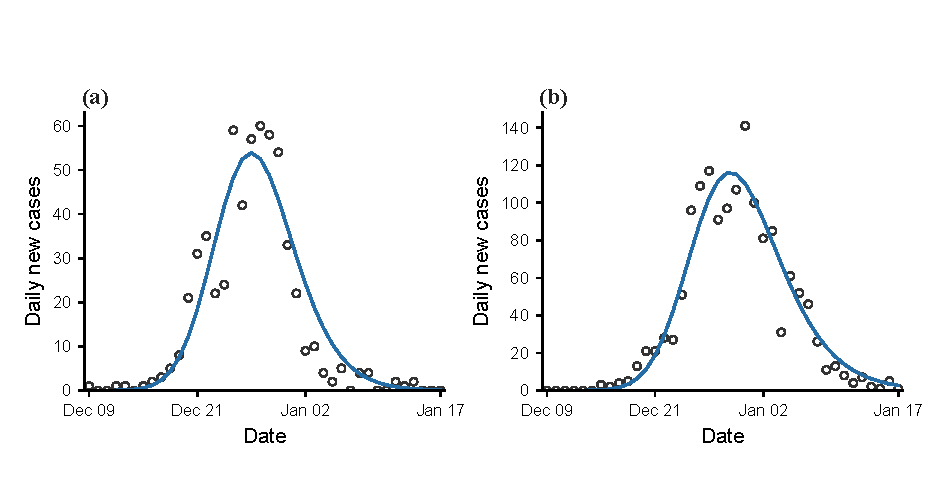
\includegraphics[width=\textwidth]{figures/layout_v5/xian_observed_fit.pdf}
\caption{西安疫情观测窗口内的日新增病例与 TDINN 重构。(a) 社区发现病例；(b) 隔离发现病例。点为观测值，实线为 TDINN 控制下的模型结果；观测窗口为 2021 年 12 月 9 日起的 40 个日区间。}
\label{fig:xian:observed-fit}
\end{figure}

\subsection{与 TDINN 的比较}
TDINN 重构是外部参照，它与仅隔离控制完成的是不同的控制任务。TDINN 控制按拟合函数同时降低接触率、提高隔离比例，既不把感染维持在某一阈值，也不要求在某一状态退出。仅隔离控制保持 $c=c_0$，在 $I$ 首次达到设计阈值 $\eta=0.002N$ 时启动，维持 $I=\eta$ 直到 $S=S_c$。常规控制始终取 $(c_0,q_0)$，是不加额外干预的反事实基准。三种策略从表~\ref{tab:xian_initial_fit}的同一初值出发，各自计算至清零时间（图~\ref{fig:xian:strategy-process}，表~\ref{tab:xian_summary}）；阈值策略下不同控制组合的比较见第~\ref{sec:joint:compare-numerics}~节。

仅隔离控制的二次成本低于 TDINN，感染却多出三个数量级，清零也晚得多（表~\ref{tab:xian_summary}）。它的 $J$ 约为 $40.77$ d，TDINN 为 $49.39$ d；它的总累计新增感染约为 $2.38\times10^6$ 人、清零时间约为 $258.1$ d，TDINN 分别约为 $2106$ 人与 $45.29$ d。$J$ 只衡量干预强度，较低的 $J$ 因而可以与大得多的感染规模并存。

差别在于阈值策略把有效再生数维持在 $1$，而 TDINN 把它压到 $1$ 以下。常规控制下 $R_e(0)\approx4.43$（$R_e$ 的定义见第~\ref{sec:model:strategy}~节），感染迅速增长。TDINN 控制使 $R_e$ 较快降到 $1$ 以下，疫情在易感者仍接近全市人口时就结束了（图~\ref{fig:xian:strategy-process}(e)）。仅隔离控制在阈值控制期内保持 $R_e=1$（式\eqref{eq:model:balance}）：$I$ 停在 $\eta$，易感者不断被感染或作为未感染接触者被隔离，直到 $S$ 降到 $S_c$ 后 $I$ 才开始下降。累计感染的规模因而由退出要求决定，下一节给出它的下界。

\begingroup
\renewcommand{\topfraction}{0.9}
\renewcommand{\textfraction}{0.1}
\begin{figure}[htbp]
\centering
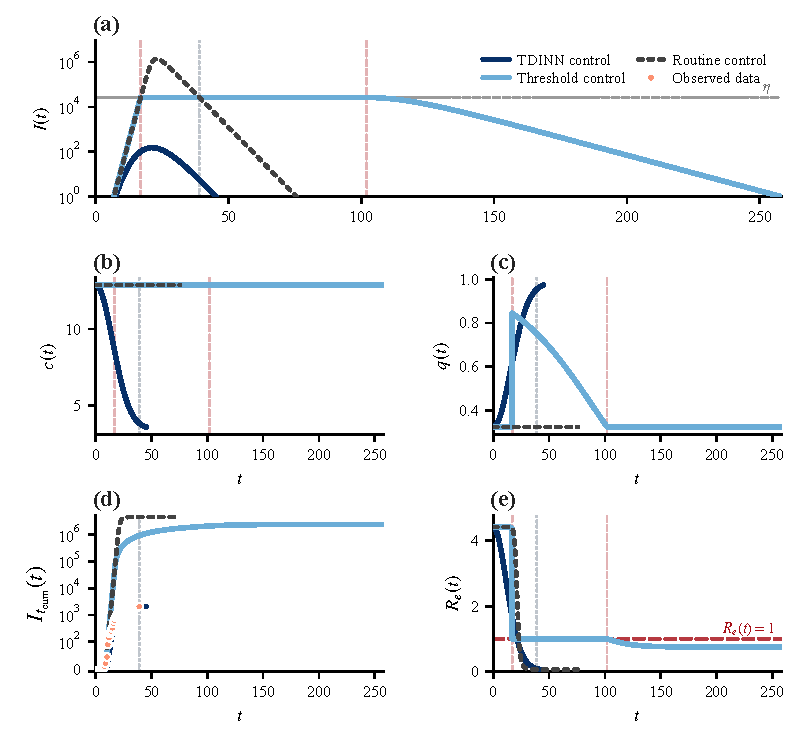
\includegraphics[width=135mm]{figures/layout_v5/xian_strategy_process.pdf}
\caption{$\eta=0.002N$ 时三种策略的全过程比较。(a) 社区感染者人数 $I(t)$，对数纵轴；(b) 接触率 $c(t)$；(c) 隔离比例 $q(t)$；(d) 总累计新增感染 $\Itcum(t)$，对称对数纵轴（线性区阈值为 $100$ 人），散点为观测累计量；(e) 有效再生数 $R_e(t)$，水平虚线为 $R_e=1$。各轨迹画至自身的清零时间，$t$ 以天计；浅红色竖虚线标记控制启动与退出，灰色竖点线标记观测窗口结束。}
\label{fig:xian:strategy-process}
\end{figure}

\begin{table}[htbp]
\centering\small
\setlength{\tabcolsep}{3.5pt}
\renewcommand{\arraystretch}{1.25}
\begin{threeparttable}
\caption{西安参数下三种策略的比较}
\label{tab:xian_summary}
\begin{tabular*}{\linewidth}{@{\extracolsep{\fill}}lS[table-format=7.0]S[table-format=7.0]S[table-format=3.2]S[table-format=2.4]@{}}
\toprule
策略 & {\shortstack{社区感染峰值\\（人）}} & {\shortstack{总累计新增感染\\（人）}} & {\shortstack{清零时间\\（d）}} & {$J$（d）}\\
\midrule
TDINN 控制 & 153 & 2106 & 45.29 & 49.3894\\
仅隔离控制 & 26326 & 2377943 & 258.10 & 40.7686\\
常规控制 & 1377552 & 4587183 & 75.57 & 0.0000\\
\bottomrule
\end{tabular*}
\begin{tablenotes}[flushleft]\footnotesize
\item 注：$\eta=0.002N$；各策略计算至自身的清零时间，人数取整。TDINN 的 $J$ 从初始时刻计至清零时间，仅隔离控制的 $J$ 只计阈值控制期。仅隔离控制的启动时刻、退出时刻与控制时长分别为 $16.90$、$101.97$、$85.07$ d。补充材料第~\ref{sec:sup:population}~节所用的 TDINN 参照值为峰值 $152.55$、总累计 $2105.63$、清零时间 $45.29$ d、$J=49.39$。
\end{tablenotes}
\end{threeparttable}
\end{table}

\FloatBarrier
\endgroup
\subsection{低阈值与退出的代价}
\label{sec:xian:threshold-scale}
设计阈值 $\eta=0.002N$ 只是一个情景（量级参考见补充材料第~\ref{sec:sup:threshold-scale}~节）；阈值越低，控制时长越长（命题~\ref{prop:threshold-tradeoff}），且近似与阈值成反比。原因是阈值控制期内 $S$ 的下降速率 $c_0\eta(S-\bar S)/N$ 与 $\eta$ 成正比，而退出仍要求 $S$ 降到同一个 $S_c$：式\eqref{eq:s1:t2}中，$\Delta t$ 等于 $N/(c_0\eta)$ 乘一个只通过启动状态 $S^*$ 依赖 $\eta$ 的对数因子。西安参数下，$\eta/N$ 从 $0.01$ 降到 $0.0001$ 时，控制时长由 $16.6$ d 增至 $1711$ d，与反比关系相符（补充表~\ref*{tab:sup:eta}，补充图~\ref{fig:xian_eta_sens}）。若把阈值降到 TDINN 的社区感染峰值 $152.55$ 人，控制时长约为 $40.5$ 年（补充图~\ref{fig:xian_heatmaps}）。

在群体免疫阈值退出本身就要求大量感染，任何控制组合都绕不开。由命题~\ref{prop:exit-infection-lower-bound}，从初始时刻到退出时刻的累计新增感染满足
\[
\Itcum(t_2)\ge\beta(S_0-S_c)\approx1.53\times10^6,
\]
已远高于 TDINN 在其清零时间的约 $2106$ 人。因此，在本模型、全市人口与这组参数下，像 TDINN 那样低的累计感染与在 $S_c$ 退出不相容。改变控制组合可以降低二次成本（表~\ref{tab:joint:compare}），却不能降低这一下界。

这些长时结果是固定参数、全市人口下的模型外推。传播参数来自观测窗口内的拟合，那时 $S(t)\approx N$；退出却要求 $S$ 降到 $S_c$，所以控制时长与感染规模都取决于参与混合的人口规模。完整的阈值与接触率扫描见补充材料第~\ref{sec:sup:xian}~节。

\subsection{有效人口}
\label{sec:dominance}
\label{sec:dom:region}
全市结果依赖有效混合人口 $N_{\rm eff}$，而这次疫情的 $N_{\rm eff}$ 未知。补充材料用一组人口情景考察这种依赖：取 $N=N_{\rm eff}$、$S_0=N-I_0$，沿用全市拟合的绝对初值 $I_0$ 与传播参数，不重新拟合。初始感染比例 $I_0/N$ 因而随人口改变；命题~\ref{prop:scaling}固定的是归一化初值，它给出的规模不变性不能直接套用。

TDINN 轨迹本身给出有效人口的一个必要下界。易感者离开 $S$ 只有三条去路：成为社区感染者、成为隔离感染者，或作为未感染接触者被隔离。记重构轨迹在其清零时间的社区与隔离累计新增感染为 $I_{\rm cum}^{\rm T}$、$I_{q_{\rm cum}}^{\rm T}$。
\begin{proposition}
\label{prop:dom:floor}
在 $S_q(0)=0$ 的无回流模型中，能够容纳给定重构轨迹的有效人口须满足
\begin{equation}
N_{\rm eff}\ge N_{\rm floor}:=
 I_{\rm cum}^{\rm T}+\frac{I_{q_{\rm cum}}^{\rm T}}{\beta}.
\label{eq:dom:Nfloor}
\end{equation}
\end{proposition}
\begin{proof}
由式\eqref{eq:count-identities}，$S_q(T)=(1-\beta)I_{q_{\rm cum}}(T)/\beta$。易感者的流出由上述三部分组成，故
\[
S_0-S(T)=I_{\rm cum}(T)+I_{q_{\rm cum}}(T)+S_q(T)
=I_{\rm cum}(T)+\frac{I_{q_{\rm cum}}(T)}\beta.
\]
再由 $S(T)\ge0$ 与 $S_0\le N_{\rm eff}$ 即得。
\end{proof}
代入 TDINN 轨迹得 $N_{\rm floor}\approx1.06\times10^4$，约为其总累计新增感染 $2105.63$ 人的 $5.04$ 倍；多出的部分是被隔离的未感染者，其人数为累计隔离感染者的 $(1-\beta)/\beta$ 倍（式\eqref{eq:count-identities}）。这只是容纳该轨迹的必要条件，不是对 $N_{\rm eff}$ 的估计。

补充材料第~\ref{sec:sup:population}~节在这一下界以上的人口情景中，比较仅隔离控制与 TDINN 的感染峰值、成本、控制时长和清零时间。在所算的情景中，凡人口满足这一下界的，仅隔离控制的清零时间都晚于 TDINN。满足各项比较条件的人口集合是否为连续区间尚未确定。下一章讨论这些结果的含义与局限。
